\part{Binary notation}
\frame{\partpage}

\begin{frame}
	\centering
	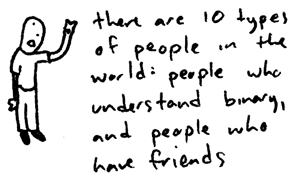
\includegraphics[width=0.7\textwidth]{10-types-of-people}
	\par\vspace{2ex}\par
	{\tiny Image credit: \url{http://www.toothpastefordinner.com}}
\end{frame}



\begin{frame}{How we write numbers}
	\begin{itemize}
		\pause\item We write numbers in \textbf{base~10}
		\pause\item We have 10 \textbf{digits}: $0, 1, 2, \dots, 8, 9$
		\pause\item When we write $6397$, we mean:
			\begin{itemize}
				\pause\item Six thousand, three hundred and ninety seven
				\pause\item (Six thousands) and (three hundreds) and (nine tens) and (seven)
				\pause\item $(6 \times 1000) + (3 \times 100) + (9 \times 10) + (7)$
				\pause\item $\left(6 \times 10^3\right)
				+ \left(3 \times 10^2\right)
				+ \left(9 \times 10^1\right)
				+ \left(7 \times 10^0\right)$
				\pause\item
				    \begin{tabular}{cccc}
				        Thousands & Hundreds & Tens & Units \\
				        6 & 3 & 9 & 7
				    \end{tabular}
			\end{itemize}
	\end{itemize}
\end{frame}

\begin{frame}{Binary}
	\begin{itemize}
		\pause\item Binary notation works the same, but is \textbf{base~2} instead of \textbf{base~10}
		\pause\item We have 2 \textbf{digits}: $0, 1$
		\pause\item When we write $10001011$ in binary, we mean: \par\pause
			$\phantom{+} \left(1 \times 2^7\right) + 
			\left(0 \times 2^6\right) + 
			\left(0 \times 2^5\right) + 
			\left(0 \times 2^4\right)$ \par
			$+ \left(1 \times 2^3\right) + 
			\left(0 \times 2^2\right) + 
			\left(1 \times 2^1\right) + 
			\left(1 \times 2^0\right)$ \par\pause
			$= 2^7 + 2^3 + 2^1 + 2^0$ \par\pause
			$= 128 + 8 + 2 + 1 \text{ (base 10)}$ \par\pause
			$= 139 \text{ (base 10)}$
	\end{itemize}
\end{frame}

\begin{frame}{Why binary?}
	\begin{itemize}
		\pause\item Modern computers are \textbf{digital}
		\pause\item Based on the flow of current in a circuit being either \textbf{on} or \textbf{off}
		\pause\item Hence it is natural to store and operate on numbers in base 2
		\pause\item The binary digits $0$ and $1$ correspond to \textbf{off} and \textbf{on} respectively
	\end{itemize}
\end{frame}

\begin{frame}{Converting to binary}
    \begin{center}
        \url{https://www.youtube.com/watch?v=OezK_zTyvAQ}
    \end{center}
\end{frame}

\begin{frame}{Bits, bytes and words}
	\begin{itemize}
		\pause\item A \textbf{bit} is a \uline{b}inary dig\uline{it}
			\begin{itemize}
				\pause\item Can store a 0 or 1 (i.e.\ a boolean value)
				\pause\item The smallest possible unit of information
			\end{itemize}
		\pause\item A \textbf{byte} is 8 \textbf{bits}
			\begin{itemize}
				\pause\item Can store a number between 0 and 255 in binary
			\end{itemize}
		\pause\item A \textbf{word} is the number of bits that the CPU works with at once
			\begin{itemize}
				\pause\item 32-bit CPU: 32 bits = 1 word
				\pause\item 64-bit CPU: 64 bits = 1 word
			\end{itemize}
		\pause\item An $n$-bit word can store a number between 0 and $2^{n} - 1$
			\begin{itemize}
				\pause\item $2^{16}-1 = 65,535$
				\pause\item $2^{32}-1 = 4,294,967,295$
				\pause\item $2^{64}-1 = 18,446,744,073,709,551,615$
			\end{itemize}
	\end{itemize}
\end{frame}

\begin{frame}{Other units}
    \begin{itemize}
        \pause\item A \textbf{nibble} is 4 \textbf{bits}
        \pause\item A \textbf{kilobyte} is 1000 or 1024 \textbf{bytes}
            \begin{itemize}
                \pause\item $10^3 = 1000 \approx 1024 = 2^{10}$
            \end{itemize}
        \pause\item A \textbf{megabyte} is 1000 or 1024 \textbf{kilobytes}
        \pause\item A \textbf{gigabyte} is 1000 or 1024 \textbf{megabytes}
        \pause\item A \textbf{terabyte} is 1000 or 1024 \textbf{gigabytes}
        \pause\item $\dots$
    \end{itemize}
\end{frame}

\newcommand{\carry}[1]{\uncover<#1->{$_1$}}
\newcommand{\nocarry}[1]{\phantom{$_1$}}

\begin{frame}{Addition with carry}
	In base 10:
	\begin{center}
		\begin{tabular}{lllll}
			& 1 & 2 & 3 & 4 \\
			+ & 5\nocarry{4} & 6\carry{3} & 7\carry{2} & 8\nocarry{1} \\\hline
			& \uncover<5->{6} & \uncover<4->{9} & \uncover<3->{1} & \uncover<2->{2}
		\end{tabular}
	\end{center}
\end{frame}

\begin{frame}{Addition with carry}
	In base 2:
	\begin{center}
		\fbox{$1 + 1 = 10$ \qquad $1 + 1 + 1 = 11$}
		
		\vspace{2ex}
		
		\begin{tabular}{lllllllll}
			& 0 & 1 & 1 & 0 & 1 & 1 & 1 & 0 \\
			+ &
				0\carry{8} &
				0\carry{7} &
				1\nocarry{6} &
				0\carry{5} &
				0\carry{4} &
				1\carry{3} &
				1\nocarry{2} &
				1 \\\hline
			&
				\uncover<9->{1} &
				\uncover<8->{0} &
				\uncover<7->{0} &
				\uncover<6->{1} &
				\uncover<5->{0} &
				\uncover<4->{1} &
				\uncover<3->{0} &
				\uncover<2->{1}
		\end{tabular}
	\end{center}
\end{frame}

\begin{frame}{Hexadecimal notation}
	\begin{columns}
		\begin{column}{0.32\textwidth}
			\begin{itemize}
				\pause\item Other number bases than 2 and 10 are also useful
				\pause\item Hexadecimal is \textbf{base 16}
				\pause\item Uses extra digits:
					\begin{itemize}
						\item \texttt{A}=10, \texttt{B}=11, ..., \texttt{F}=15
					\end{itemize}
			\end{itemize}
		\end{column}
		\pause
		\begin{column}{0.64\textwidth}
			\begin{tabular}{rl|rl|rl}
				\textbf{Hex} & \textbf{Dec} & \textbf{Hex} & \textbf{Dec} & \textbf{Hex} & \textbf{Dec} \\
				\texttt{00} & 0             & \texttt{10} & 16            & \texttt{F0} & 240           \\
				\texttt{01} & 1             & \texttt{11} & 17            & \texttt{F1} & 241           \\
				$\vdots$ & $\vdots$         & $\vdots$ & $\vdots$         & $\vdots$ & $\vdots$         \\
				\texttt{09} & 9             & \texttt{19} & 25            & \texttt{F9} & 249           \\
				\texttt{0A} & 10            & \texttt{1A} & 26            & \texttt{FA} & 250           \\
				\texttt{0B} & 11            & \texttt{1B} & 27            & \texttt{FB} & 251           \\
				\texttt{0C} & 12            & \texttt{1C} & 28            & \texttt{FC} & 252           \\
				\texttt{0D} & 13            & \texttt{1D} & 29            & \texttt{FD} & 253           \\
				\texttt{0E} & 14            & \texttt{1E} & 30            & \texttt{FE} & 254           \\
				\texttt{0F} & 15            & \texttt{1F} & 31            & \texttt{FF} & 255           
			\end{tabular}
		\end{column}
	\end{columns}
\end{frame}
